\part{Space-Time Data}
\label{cha:Spatio-Time}

\chapter{Displaying Spatiotemporal Data: Introduction}
\label{cha:introductionST}

Space-time datasets are indexed both in space and in time. The
data may consist of a spatial vector object (for example, points
or polygons) or raster data at different times. The first case is
representative of data from fixed sensors providing measurements
abundant in time but sparse in space. The second case is the
typical format of satellite imagery, which produces high spatial
resolution data sparse in time \cite{Pebesma2012}.

There are several visualization approaches of space-time data
trying to cope with the four dimensions of the data
\cite{Cressie.Wikle2011}. 

On the one hand, the data can be conceived as a collection of
snapshots at different times. These snapshots can be displayed as a
sequence of frames to produce an animation, or can be printed on one
page with different panels for each snapshot using the small-multiple
technique described repeatedly in previous chapters.

On the other hand, one of the two spatial dimensions can be collapsed
through an appropriate statistic (for example, mean or standard
deviation) to produce a space-time plot (also known as a Hovmöller
diagram). The axes of this graphic are typically longitude or latitude
as the x-axis, and time as the y-axis, with the value of the
spatial-averaged value of the raster data represented with color.

Finally, the space-time object can be reduced to a multivariate
time series (where each location is a variable or column of the
time series) and displayed with the time series visualization
techniques described in the Part \ref{part:Time}. This
approach is directly applicable to space-time data sparse in space
(for example, point measurements at different times). However, it is
mandatory to use aggregation in the case of raster data. In this
case, the multivariate time series is composed of the evolution of
the raster data averaged along a certain direction.
 
The next chapters, focused on raster space-time data (Chapter
\ref{cha:rasterST}) and point space-time data (Chapter
\ref{cha:pointsST}), illustrate with examples how to produce
animations, multipanel graphics, hovmöller diagrams, and
time-series with \textsf{R}.

% \hline 
\section{Packages}
\label{sec:spacetime-packages}

The CRAN Tasks View ``Handling and Analyzing Spatiotemporal
Data''\footnote{\url{http://cran.r-project.org/web/views/SpatioTemporal.html}}
summarizes the packages for reading, vizualizing, and analyzing
space-time data. This section provides a brief introduction to the
\texttt{spacetime}, \texttt{raster}, and \texttt{rasterVis}
packages. Most of the information has been extracted from their
vignettes, webpages, and help pages. You should read them for detailed
information.

\subsection{spacetime}
\label{sec:spacetime}
\index{Packages!spacetime@\texttt{spacetime}} The \texttt{spacetime}
package \cite{Pebesma2012} is built upon the classes and methods for
spatial data from the \texttt{sp} package , and for time series data
from the \texttt{xts} package. It defines classes to represent four
space-time layouts:
\begin{enumerate}
\item \texttt{STF}, \texttt{STFDF}: full space-time grid of
  observations for spatial features and observation time, with all
  space-time combinations.
\item \texttt{STS}, \texttt{STSDF}: sparse grid layout, stores only
  the non-missing space-time combinations on a lattice
\item \texttt{STI}, \texttt{STIDF}: irregular layout, time and space
  points of measured values have no apparent organisation.
\item \texttt{STT}, \texttt{STTDF}: simple trajectories.
\end{enumerate}

Moreover, \texttt{spacetime} provides several methods for the
following classes:
\begin{itemize}
\item \texttt{stConstruct}, \texttt{STFDF}, and \texttt{STIDF} create
  objects from single or multiple tables.
\item \texttt{as} coerces to other spatiotemporal objects, xts,
  Spatial, matrix, or data.frame.
\item \texttt{[[} selects or replaces data values.
\item \texttt{[} selects spatial or temporal subsets, and data
  variables.
\item \texttt{over} retrieves index or data values of one object at the
  locations and times of another.
\item \texttt{aggregate} aggregates data values over particular
  spatial, temporal, or spatiotemporal domains.
\item \texttt{stplot} creates spatiotemporal plots. It is able to
  produce multi-panel plots, space-time plots, animations, and time
  series plots.
\end{itemize}


\subsection{raster}
\label{sec:rasterST}
\index{Packages!raster@\texttt{raster}}

The \texttt{raster} package \cite{Hijmans2013} is able to add time
information associated with layers of a \texttt{RasterStack} or
\texttt{RasterBrick} object with the \texttt{setZ} function. This
information can be extracted with \texttt{getZ}.

If a \texttt{Raster*} object includes this information, the
\texttt{zApply} function can be used to apply a function over a time
series of layers of the object.


\subsection{rasterVis}
\label{sec:rastervisST}
\index{Packages!rasterVis@\texttt{rasterVis}}

\texttt{rasterVis} \cite{Perpinan.Hijmans2013} provides three methods
to display spatiotemporal rasters:
\begin{enumerate}
\item \texttt{hovmoller} produces Hovmöller diagrams
  \cite{Hovmoeller1949a}. The axes of this kind of diagram are
  typically longitude or latitude (x-axis) and time (ordinate or
  y-axis) with the value of some aggregated field represented through
  color. However, the user can define the direction with
  \texttt{dirXY} and the summary function with \texttt{FUN}.
\item \texttt{horizonplot} creates horizon graphs \cite{Few2008}, with
  many time series displayed in parallel by cutting the vertical range
  into segments and overplotting them with color representing the
  magnitude and direction of deviation. Each time series corresponds
  to a geographical zone defined with \texttt{dirXY} and averaged with
  \texttt{zonal}.
\item \texttt{xyplot} displays conventional time series plots. Each
  time series corresponds to a geographical zone defined with
  \texttt{dirXY} and aggregated with \texttt{zonal}.
\end{enumerate}

On the other hand, the \texttt{histogram}, \texttt{densityplot}, and
\texttt{bwplot} methods accept a \texttt{FUN} argument to be applied
to the \texttt{z} slot of \texttt{Raster*} object (defined by
\texttt{setZ}). The result of this function is used as the grouping
variable of the plot to create different panels.

\section{Further Reading}
\label{cha:further-reading-spatiotime}

\begin{itemize}

\item \cite{Cressie.Wikle2011} is a systematic approach to key
  quantitative techniques on statistics for spatiotemporal data.
  The book begins with separate treatments of temporal data and
  spatial data, and later combines these concepts to discuss
  spatiotemporal statistical methods. There is a chapter devoted
  to exploratory methods, including visualization techniques.

\item \cite{Pebesma2012} presents the \texttt{spacetime} package, which
  implements a set of classes for spatiotemporal data. This paper
  includes examples that illustrate how to import, subset, coerce, and
  export spatiotemporal data, proposes several visualization methods,
  and discusses spatiotemporal geostatistical interpolation.

\item \cite{Slocum.McMaster.ea2005} (previously cited in Chapter
  \ref{cha:further-reading-spatial}) includes a chapter about map
  animation, discussing several approaches for displaying
  spatiotemporal data.

\item \cite{Hengl2009} (previously cited in Chapter
  \ref{cha:further-reading-spatial}) includes a working example
  with spatiotemporal data to illustrate space-time variograms
  and interpolation.

\item \cite{Harrower.Fabrikant2008} explore the role of animation in
  geographic visualization and outline the challenges, both conceptual
  and technical, involved in the creation and use of animated maps.

\item The CRAN Tasks View ``Handling and Analyzing Spatiotemporal
  Data''
  \footnote{\url{http://cran.r-project.org/web/views/SpatioTemporal.html}}
  summarizes the packages for reading, vizualizing, and analyzing
  space-time data.  The R-SIG-Geo mailing
  list\footnote{\url{https://stat.ethz.ch/mailman/listinfo/R-SIG-Geo/}}
  is a powerful resource for obtaining help.

\end{itemize}



\chapter{Spatiotemporal Raster Data}
\label{cha:rasterST}


\section{Introduction}
\label{sec-1}

A space-time raster dataset is a collection of raster layers indexed
by time, or in other words, a time series of raster maps. The \texttt{raster}
package defines the classes \texttt{RasterStack} and \texttt{RasterBrick} to build
multilayer rasters. The index of the collection can be set with the
function \texttt{setZ} (which is not restricted to time indexes). The
\texttt{rasterVis} packages provide several methods to display space-time
rasters.

\subsection{Data}
\label{sec-1-1}
Throughout this chapter we will work with a multilayer raster of daily
solar radiation estimates from CM SAF (section \ref{sec:CMSAF}) falling in
the region of Galicia (north of Spain) during 2011. These data are
arranged in a \texttt{RasterBrick} with 365 layers using \texttt{brick} and time
indexed with \texttt{setZ}.

\index{Packages!raster@\texttt{raster}}
\index{Packages!zoo@\texttt{zoo}}
\index{Packages!rasterVis@\texttt{rasterVis}}
\index{setZ@\texttt{setZ}}

\lstset{language=R,numbers=none}
\begin{lstlisting}
library(raster)
library(zoo)
library(rasterVis)

SISdm <- brick('data/SISgal')

timeIndex <- seq(as.Date('2011-01-01'), by='day', length=365)
SISdm <- setZ(SISdm, timeIndex)
names(SISdm) <- format(timeIndex, '%a_%Y%m%d')
\end{lstlisting}
\section{Level Plots}
\label{sec-2}

This multilayer raster can be displayed with each snapshot in a
panel using the small-multiple technique. The problem with this
approach is that only a limited number of panels can be correctly
displayed on one page. In this example, we print the first 12
days of the sequence (Figure \ref{fig:SISdm}).

\index{levelplot@\texttt{levelplot}}

\lstset{language=R,numbers=none}
\begin{lstlisting}
levelplot(SISdm, layers=1:12, panel=panel.levelplot.raster)
\end{lstlisting}

\begin{figure}[htb]
\centering
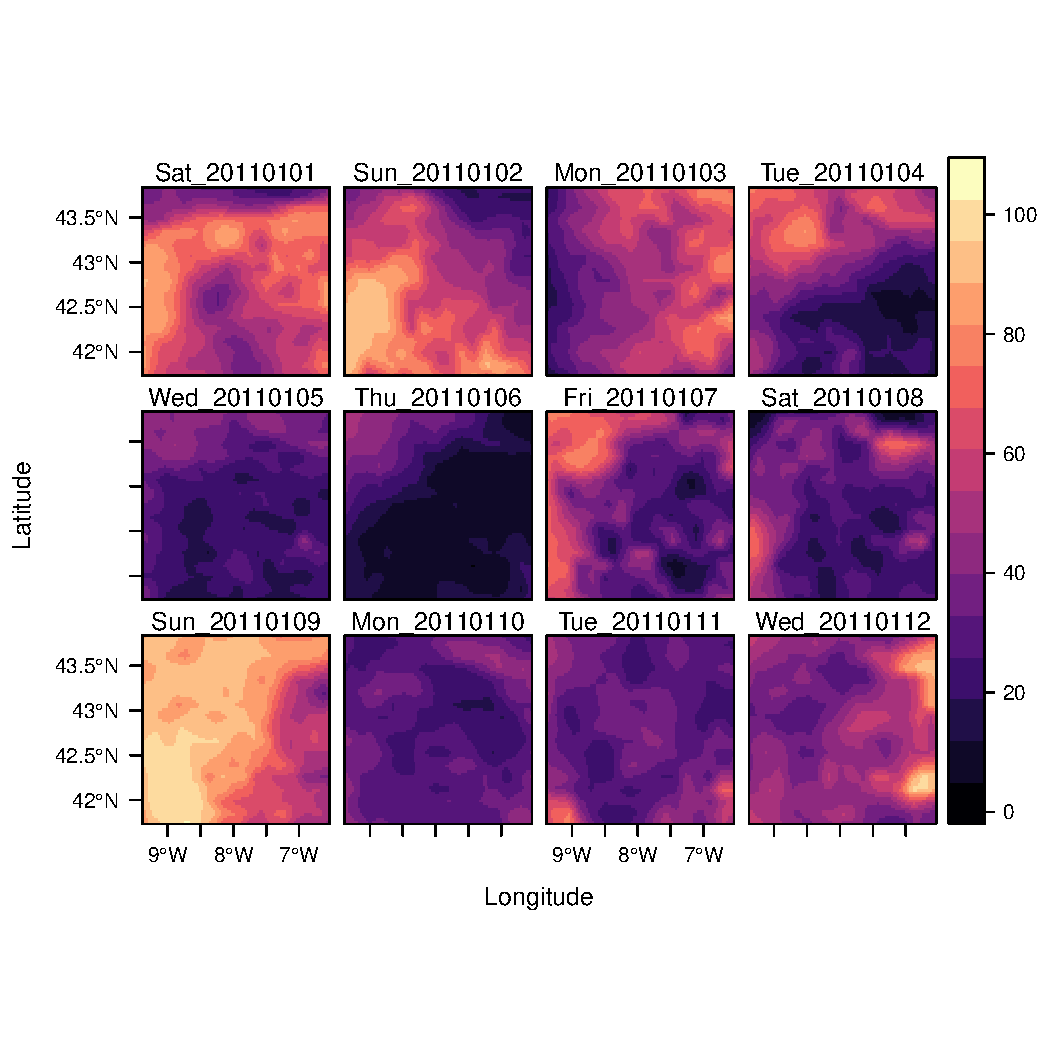
\includegraphics[width=.9\linewidth]{figs/SISdm.pdf}
\caption{\label{fig:SISdm}Level plot of daily averages of solar radiation.}
\end{figure}

When the number of layers is very high, a partial solution is to
aggregate the data, grouping the layers according to a time
condition. For example, we can build a new space-time raster with
the monthly averages using \texttt{zApply} and \texttt{as.yearmon}. This raster
can be completely displayed on one page (Figure \ref{fig:SISmm}),
although part of the information of the original data is lost in
the aggregation procedure.

\index{zApply@\texttt{zApply}}

\lstset{language=R,numbers=none}
\begin{lstlisting}
SISmm <- zApply(SISdm, by=as.yearmon, fun='mean')
\end{lstlisting}

\lstset{language=R,numbers=none}
\begin{lstlisting}
levelplot(SISmm, panel=panel.levelplot.raster)
\end{lstlisting}

\begin{figure}[htb]
\centering
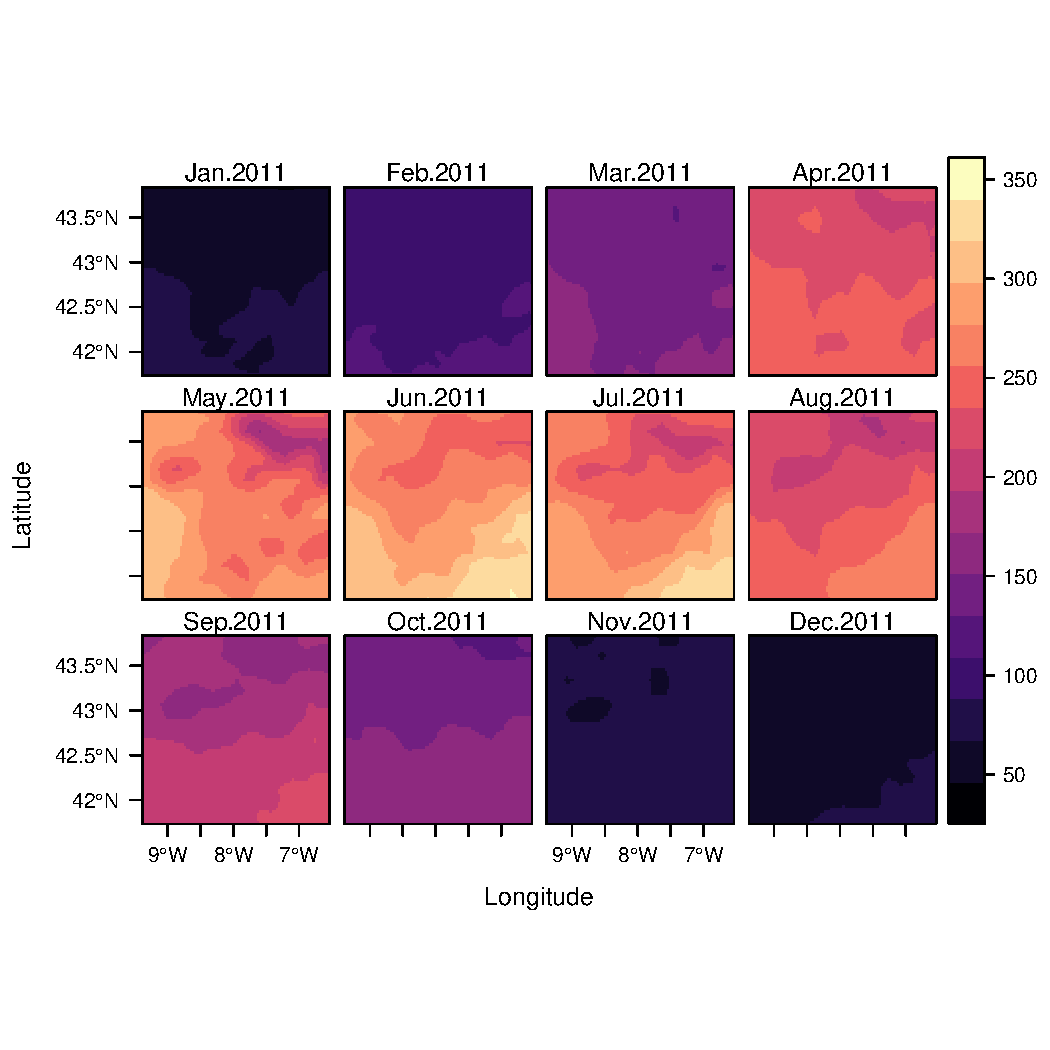
\includegraphics[width=.9\linewidth]{figs/SISmm.pdf}
\caption{\label{fig:SISmm}Level plot of monthly averages of solar radiation.}
\end{figure}
\section{Graphical Exploratory Data Analysis}
\label{sec-3}

There are other graphical tools that complement the previous maps. The
scatterplot and the matrix of scatterplots, the histogram and kernel
density plot, and the boxplot are among the most important tools in
the frame of the Exploratory Data Analysis approach. Some of them were
previously used with a spatial raster (Chapter \ref{cha:raster}). In
this section we will use the histogram (Figure \ref{fig:SISdm_hist}),
the violin plot (a combination of a boxplot and a kernel density plot)
(Figure \ref{fig:SISdm_boxplot}), and the matrix of scatterplots
(section \ref{SEC:groupVariable}, Figure \ref{fig:SISmm_splom}).

\index{histogram@\texttt{histogram}}

\lstset{language=R,numbers=none}
\begin{lstlisting}
histogram(SISdm, FUN=as.yearmon)
\end{lstlisting}

\begin{figure}[htb]
\centering
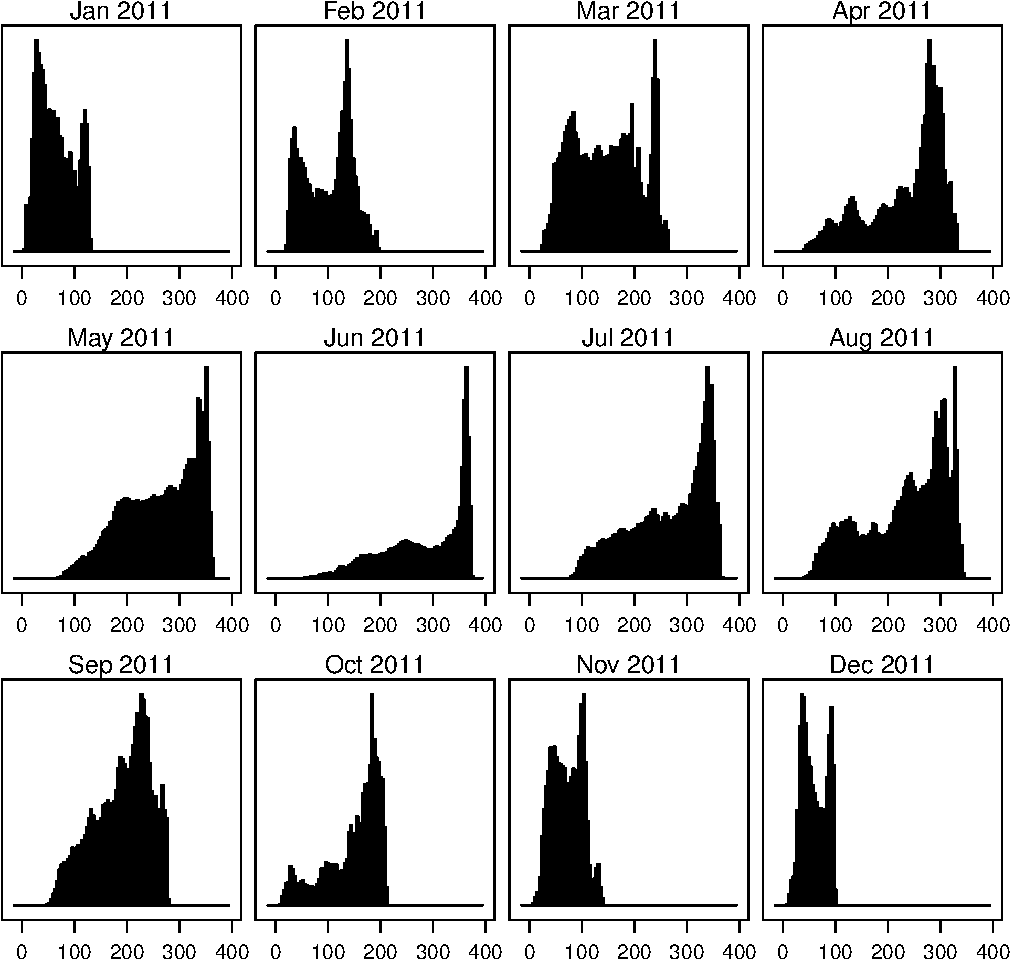
\includegraphics[width=.9\linewidth]{figs/SISdm_histogram.pdf}
\caption{\label{fig:SISdm_hist}Histogram of monthly distribution of solar radiation.}
\end{figure}


\index{bwplot@\texttt{bwplot}}
\lstset{language=R,numbers=none}
\begin{lstlisting}
bwplot(SISdm, FUN=as.yearmon)
\end{lstlisting}

\begin{figure}[htb]
\centering
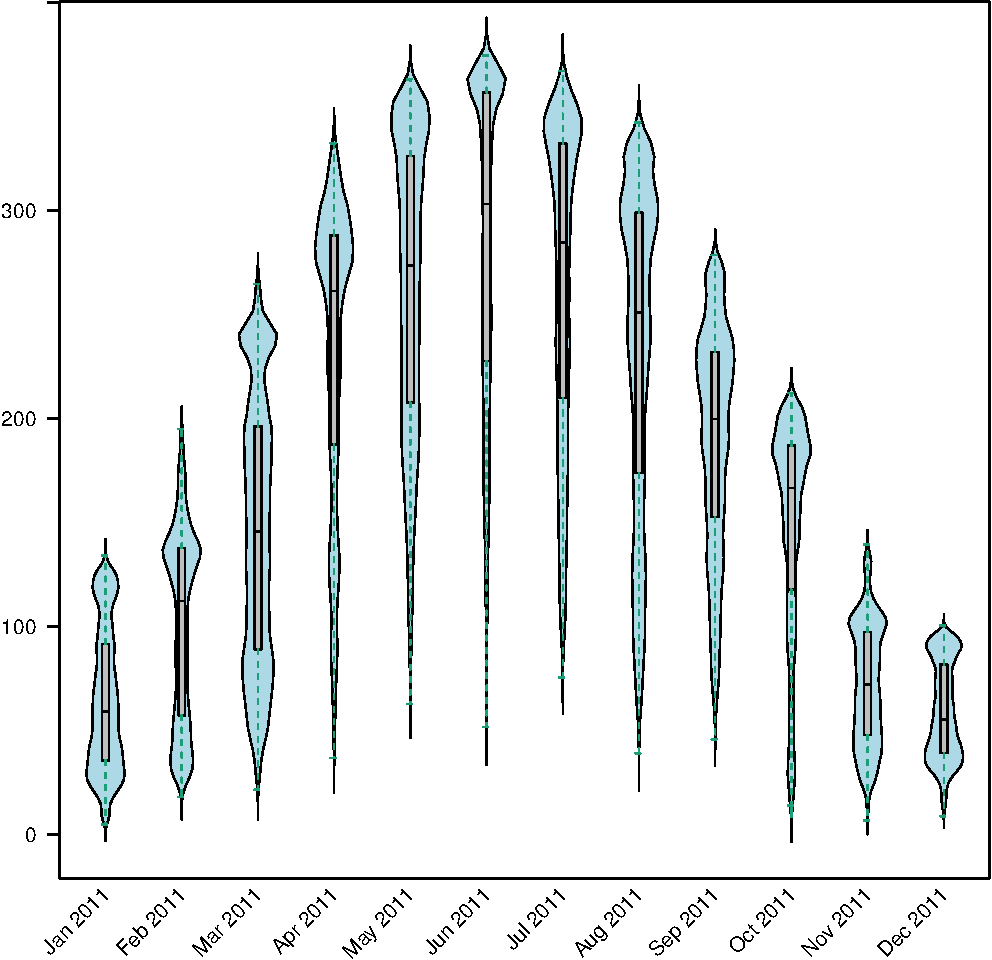
\includegraphics[width=.9\linewidth]{figs/SISdm_boxplot.pdf}
\caption{\label{fig:SISdm_boxplot}Violin plot of monthly distribution of solar radiation.}
\end{figure}

\index{splom@\texttt{splom}}

\lstset{language=R,numbers=none}
\begin{lstlisting}
splom(SISmm, xlab='', plot.loess=TRUE)
\end{lstlisting}

\begin{figure}[htb]
\centering
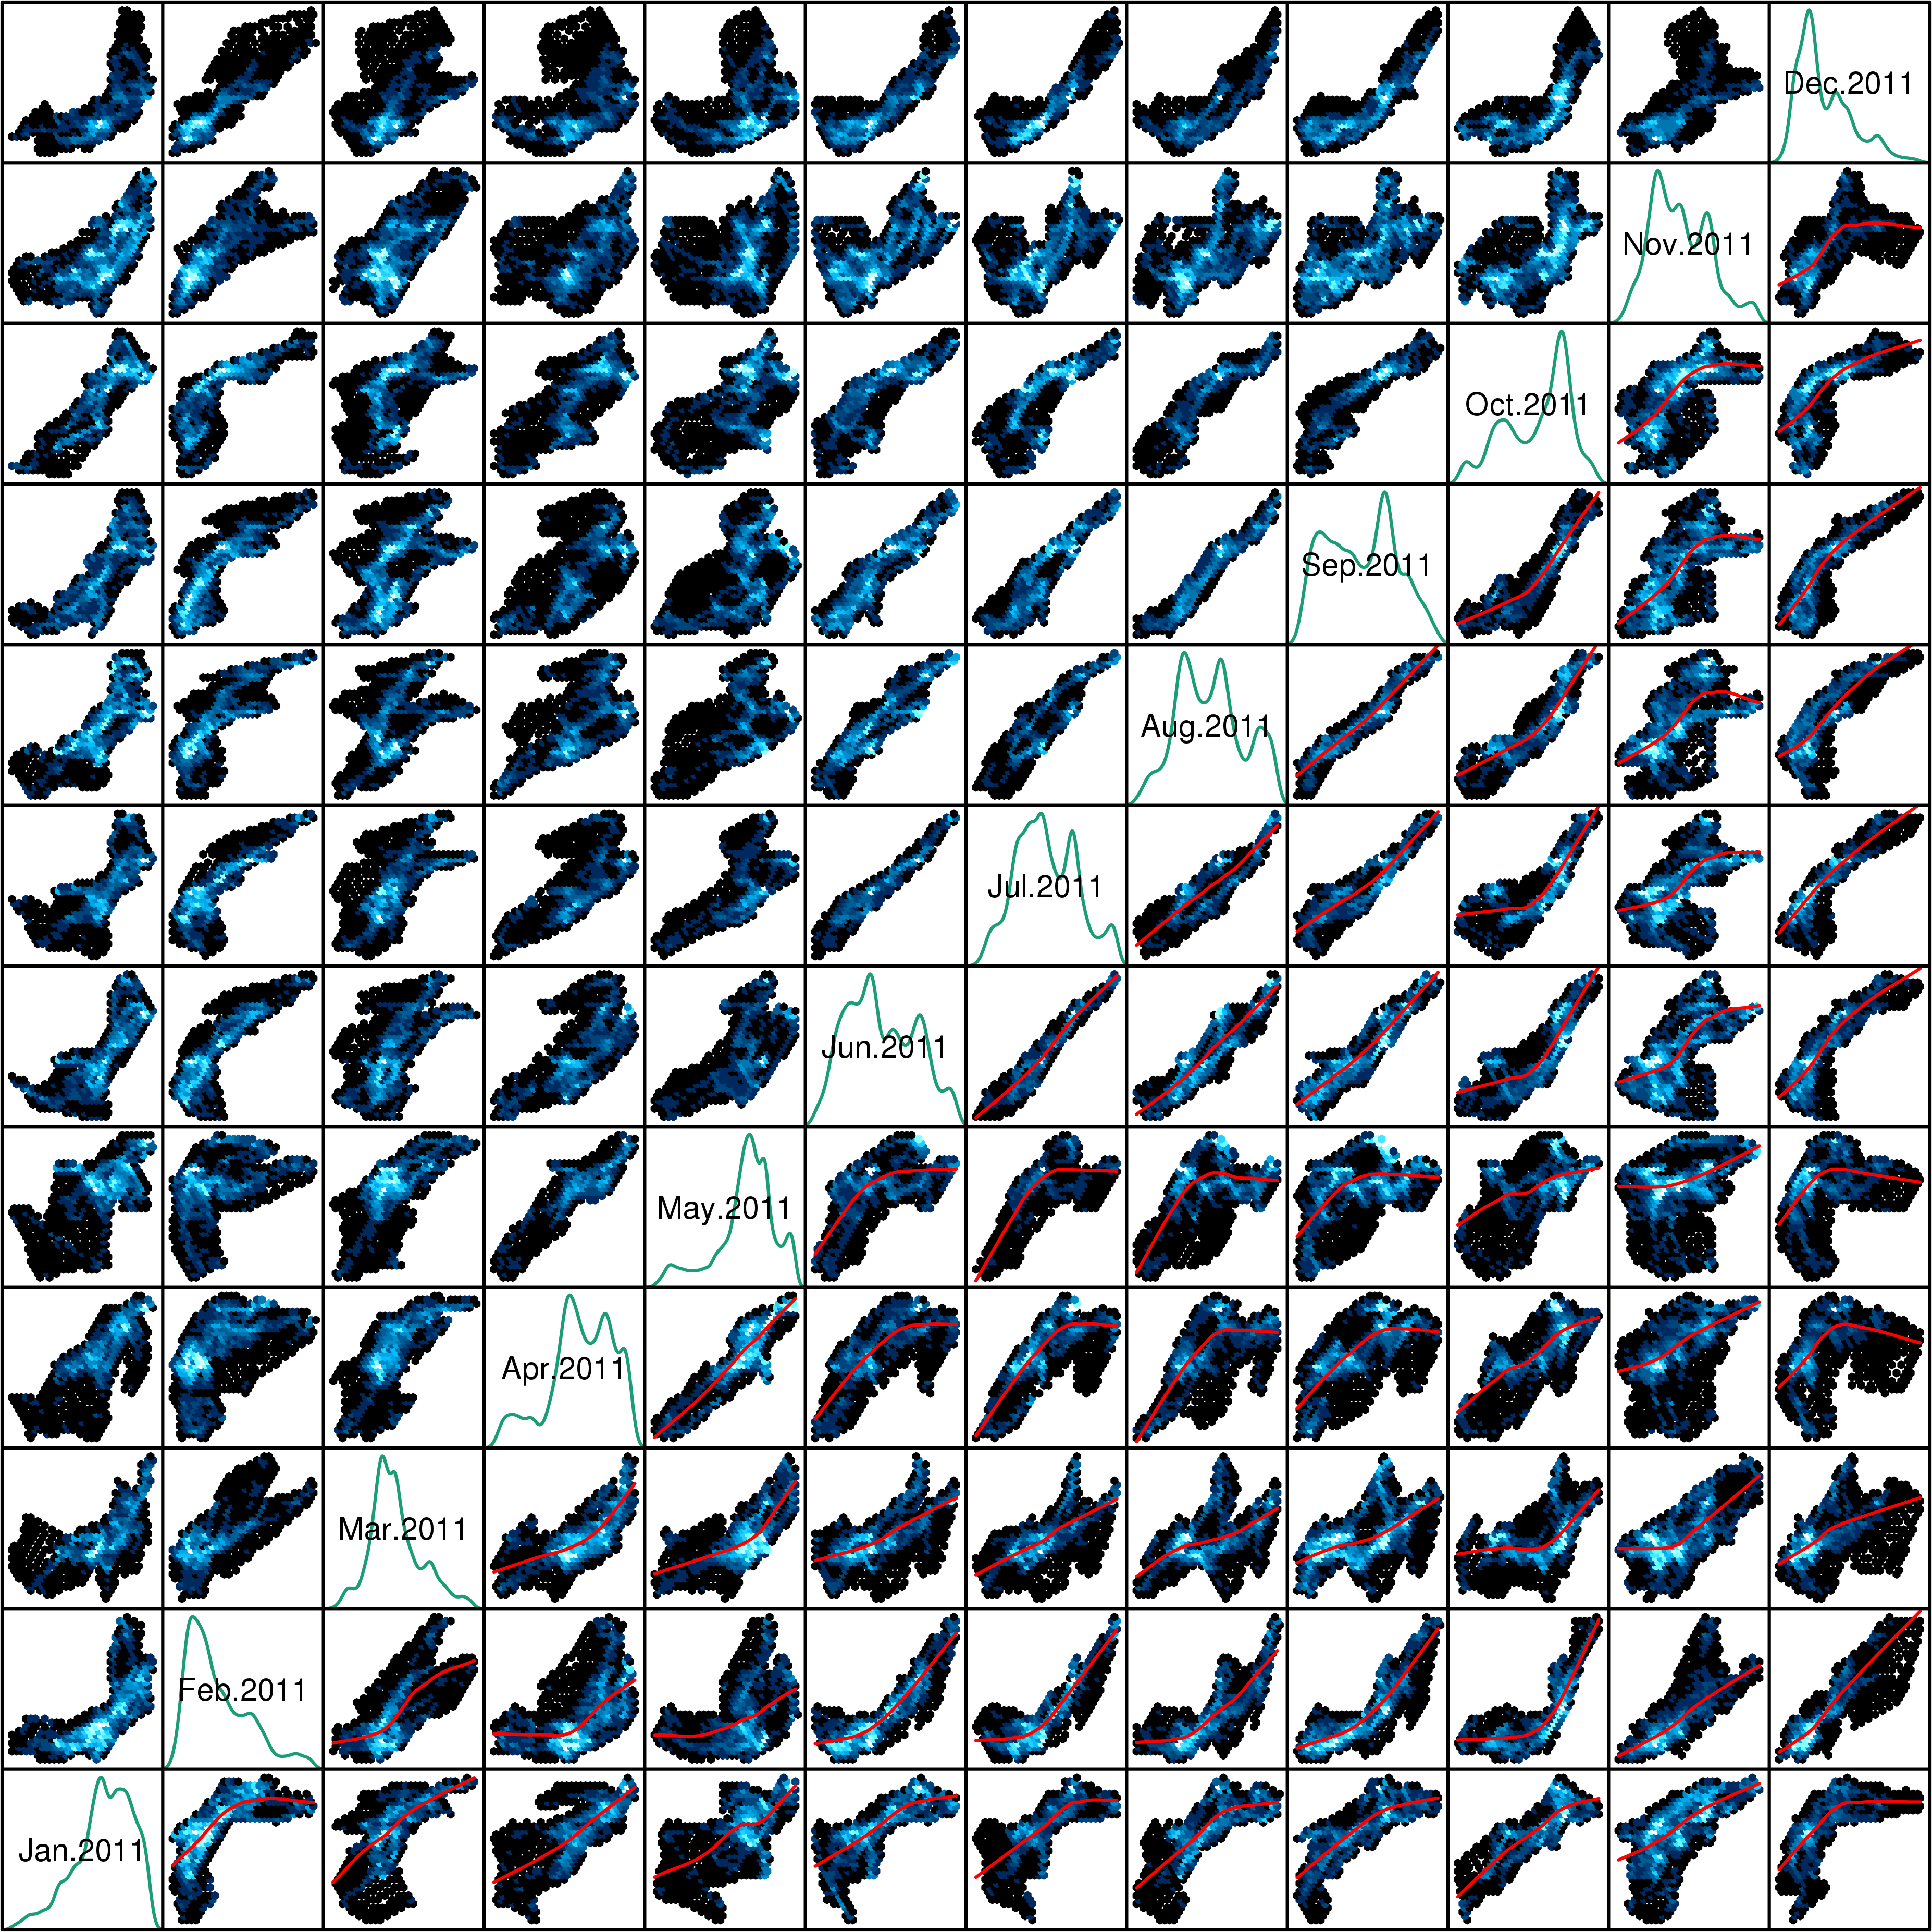
\includegraphics[width=.9\linewidth]{figs/SISmm_splom.png}
\caption{\label{fig:SISmm_splom}Scatterplot matrix of monthly averages together with their kernel density estimations in the diagonal frames.}
\end{figure}


Both the histogram and the violin plot show that daily solar
irradiation is bimodal almost every month. This is related to the
predominance of clear sky and overcast days, with several partly
cloudy days between these modes. This geographical region receives
higher irradiation levels from June to September, and both the levels
and the shape of the probability distribution contrast sharply with
the winter.

The matrix of scatterplots displays a quasilinear relationship
between the central months due to the predominance of clear sky
conditions. However, the relationships involving winter months become
strongly nonlinear due to the presence of clouds.
\section{Space-Time and Time Series Plots}
\label{sec-4}
The level plots of Figures \ref{fig:SISdm} and \ref{fig:SISmm}
display the full 3D space-time with a grid of panels where each layer
is printed. In other words, the raster is sliced, and the collection of
pieces is shown in a table. In the section \ref{sec:animationST}, this
collection of layers will be displayed sequentially like frames of a
movie to build an animation. In this section, the 3D raster is reduced
to a 2D matrix with spatial aggregation following a certain
direction. For example, Figure \ref{fig:SISdm_hovmoller_lat}
displays with colors the averaged value of the raster for each
latitude zone (using the default value of the argument \texttt{dirXY}) with
time on the vertical axis.

\index{hovmoller@\texttt{hovmoller}}

\lstset{language=R,numbers=none}
\begin{lstlisting}
hovmoller(SISdm, par.settings=BTCTheme())
\end{lstlisting}

\begin{figure}[htb]
\centering
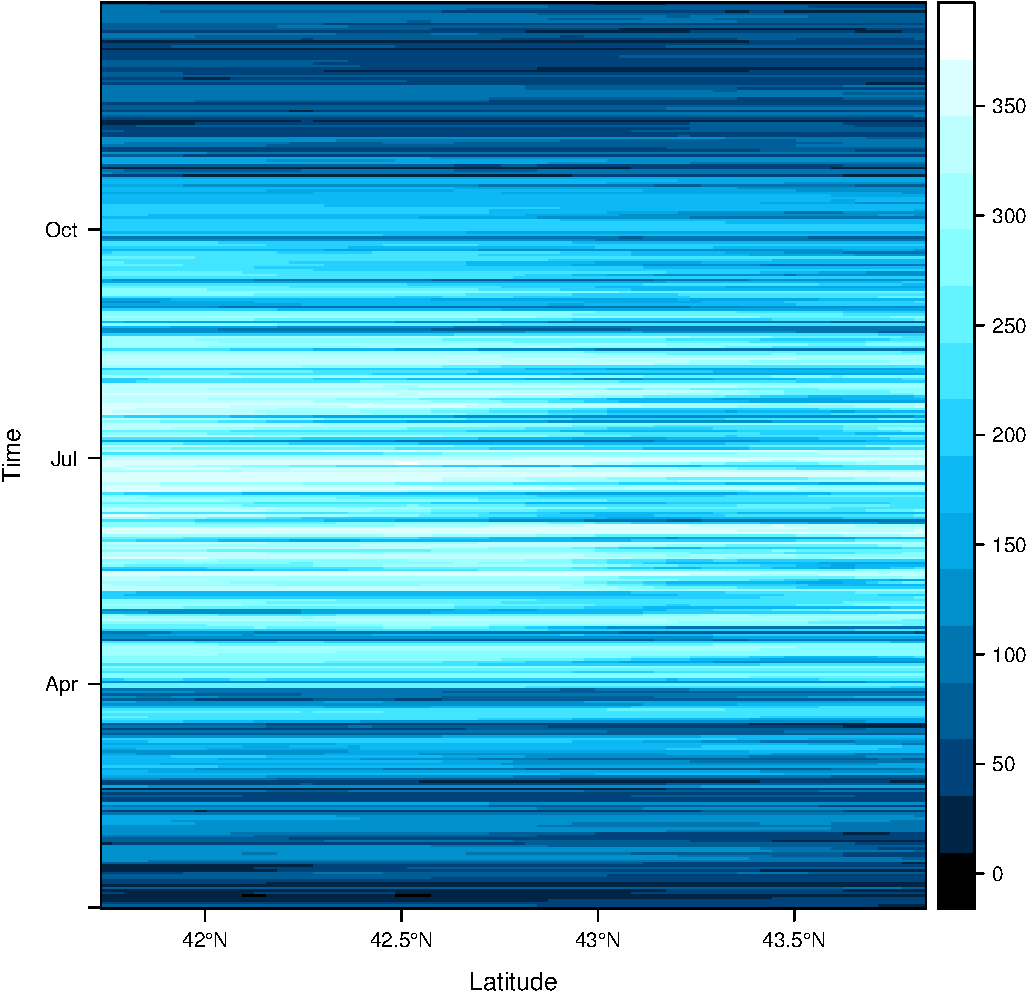
\includegraphics[width=.9\linewidth]{figs/SISdm_hovmoller_lat.pdf}
\caption{\label{fig:SISdm_hovmoller_lat}Hovmöller graphic displaying the time evolution of the average solar radiation for each latitude zone.}
\end{figure}

On the other hand, this 2D matrix can be conceived as a multivariate
time series with each aggregated zone conforming to a different variable of
the time series. This approach is followed by the \texttt{xyplot} (Figure
\ref{fig:SISmm_xyplot}) and \texttt{horizonplot} (Figure \ref{fig:SISdm_horizonplot})
methods, which reproduce the procedures described in Chapter
\ref{cha:timeHorizontalAxis} to display multivariate time series.

\index{xyplot@\texttt{xyplot}}

\lstset{language=R,numbers=none}
\begin{lstlisting}
xyplot(SISdm, digits=1, col='black', lwd=0.2, alpha=0.6)
\end{lstlisting}

\begin{figure}[htb]
\centering
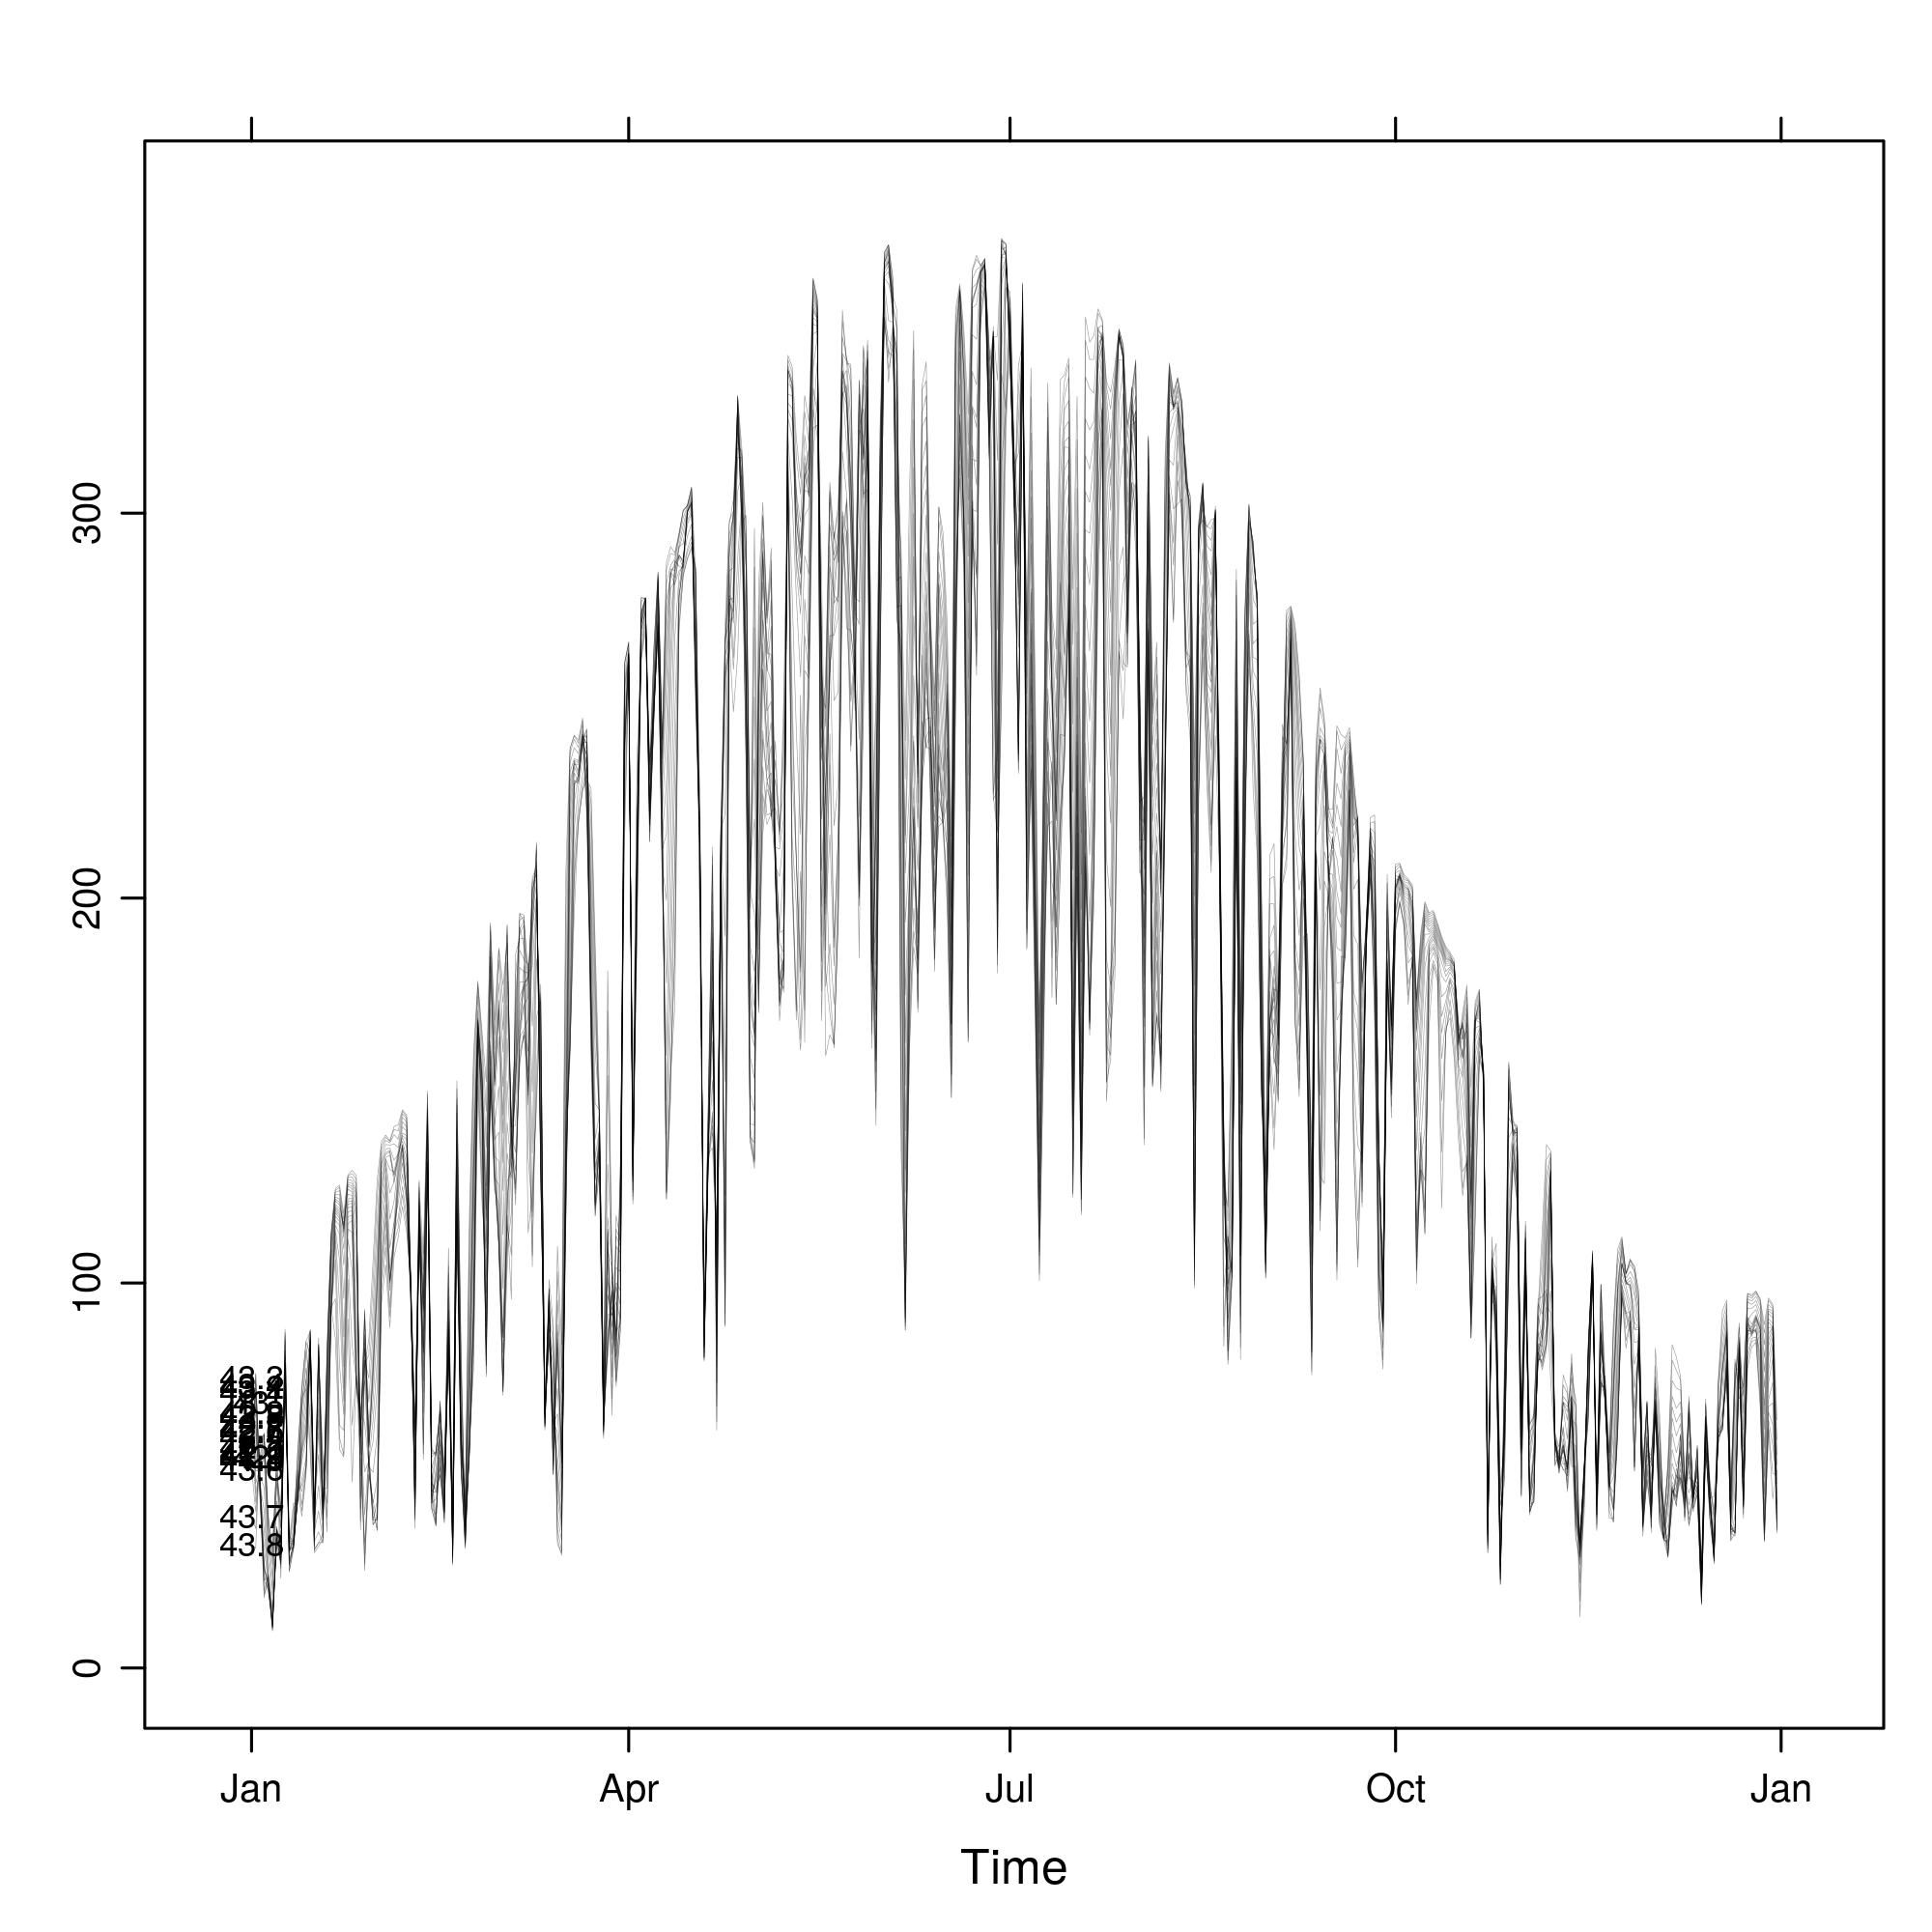
\includegraphics[width=.9\linewidth]{figs/SISmm_xyplot.png}
\caption{\label{fig:SISmm_xyplot}Time graph of the average solar radiation for each latitude zone. Each line represents a latitude band.}
\end{figure}

\index{horizonplot@\texttt{horizonplot}}

\lstset{language=R,numbers=none}
\begin{lstlisting}
horizonplot(SISdm, digits=1,
	    col.regions=rev(brewer.pal(n=6, 'PuOr')),
	    xlab='', ylab='Latitude')
\end{lstlisting}

\begin{figure}[htb]
\centering
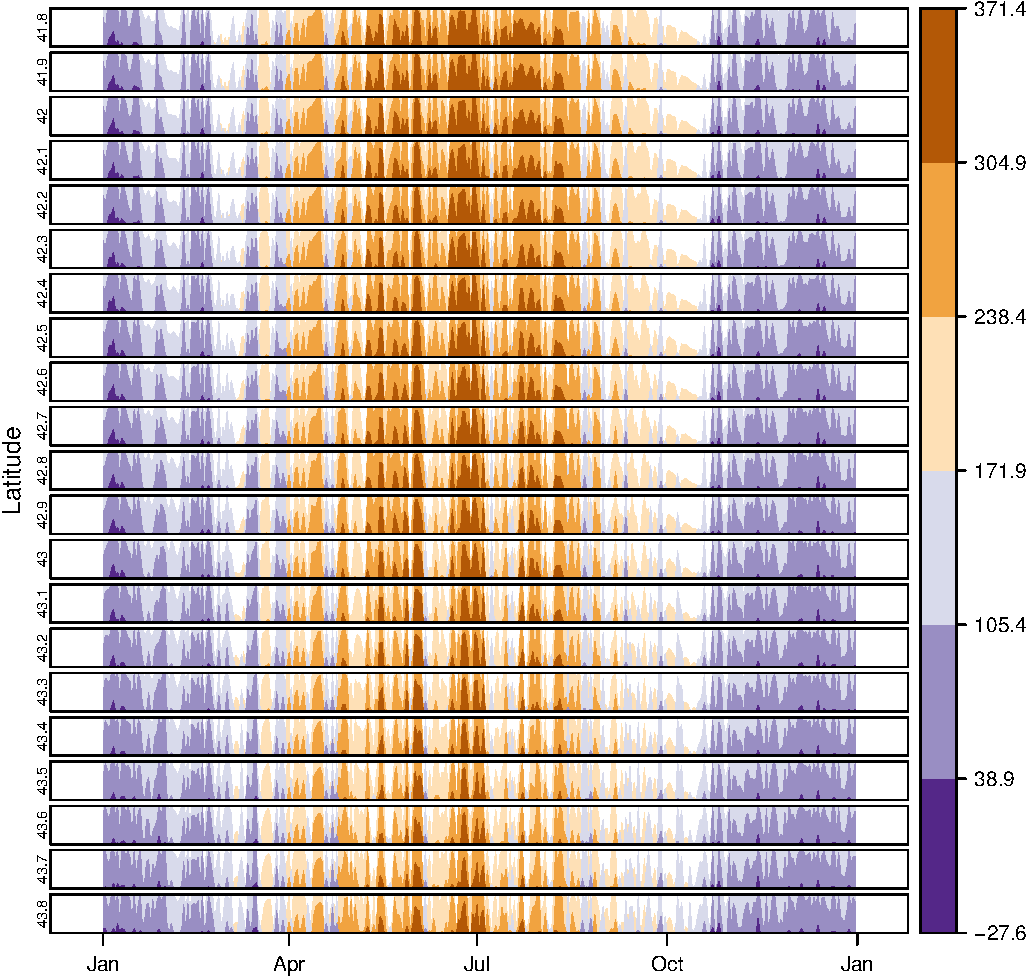
\includegraphics[width=.9\linewidth]{figs/SISdm_horizonplot.pdf}
\caption{\label{fig:SISdm_horizonplot}Horizon graph of the average solar radiation for each latitude zone.}
\end{figure}

These three figures highlight the stational behavior of the solar
radiation, with higher values during the central months. It is
interesting to note that (Figure \ref{fig:SISdm_horizonplot}) the
radiation values around the equinoxes fluctuate near the yearly
average value of each latitude region.
\section{Animation}
\label{sec-5}
\label{sec:animationST}

A different approach is to plot the individual layers of the
space-time raster sequentially as movie frames to produce an
animation. The procedure is quite simple:
\begin{itemize}
\item Plot each layer of the raster to produce a collection of graphic
files.
\item Join these files as a sequence of frames with a suitable tool (for
example, \texttt{ffmpeg}) to create a movie file\footnote{The \texttt{animation} package \cite{Xie2013} defines several functions to wrap \texttt{ffmpeg} and \texttt{convert} from ImageMagick.}\textsuperscript{,}\,\footnote{An alternative method is the \LaTeX{} animate package, which
provides an interface to create portable JavaScript-driven PDF
animations from rasterized image files.}.
\end{itemize}


The effectiveness of this visualization procedure is partly related to
the similitude between consecutive frames. If the frames of the
sequence diverge excessively from one to another, the user will
experience difficulties to perceive any relationship between them. On
the other hand, if the transitions between layers are smooth enough,
the frames will be perceived as conforming to a whole story; and,
moreover, the user will be able to spot both the stable patterns and
the important variations.

\subsection{Data}
\label{sec-5-1}
The daily solar radiation CM-SAF data do not meet the condition of
a smooth transition between layers. The changes between the consecutive
snapshots of daily radiation are too abrupt to be glued one after
another. We will work with a different dataset in this section.

The THREDSS server\footnote{\url{http://mandeo.meteogalicia.es/thredds/catalogos/WRF_2D/catalog.html}} of Meteogalicia\footnote{\url{http://www.meteogalicia.es}} provides access
through different protocols to the output of a Weather Research
and Forecasting (WRF) model, a mesoscale numerical weather
prediction system. Among the set of available variables we will
use the forecast of hourly cloud cover at low and mid levels. This
space-time raster has a time horizon of 96 hours and a spatial
resolution of 12 kilometers.

\lstset{language=R,numbers=none}
\begin{lstlisting}
cft <- brick('data/cft_20130417_0000.nc')
## use memory instead of file
cft[] <- getValues(cft)
## set projection
projLCC2d <- "+proj=lcc +lon_0=-14.1 +lat_0=34.823 +lat_1=43 +lat_2=43 +x_0=536402.3 +y_0=-18558.61 +units=km +ellps=WGS84"
projection(cft) <- projLCC2d
#set time index
timeIndex <- seq(as.POSIXct('2013-04-17 01:00:00', tz='UTC'), length=96, by='hour')
cft <- setZ(cft, timeIndex)
names(cft) <- format(timeIndex, 'D%d_H%H')
\end{lstlisting}

\subsection{Spatial Context: Administrative Boundaries}
\label{sec-5-2}
Let's provide the spatial context with the countries
boundaries, extracted from the \texttt{worldHires} database of the \texttt{maps}
and \texttt{mapdata} packages.

\index{Packages!maptools@\texttt{maptools}}
\index{Packages!mapdata@\texttt{mapdata}}
\index{Packages!maps@\texttt{maps}}
\index{Packages!rgdal@\texttt{rgdal}}
\index{map2SpatialLines@\texttt{map2SpatialLines}}
\index{spTransform@\texttt{spTransform}}

\lstset{language=R,numbers=none}
\begin{lstlisting}
library(maptools)
library(rgdal)
library(maps)
library(mapdata)


projLL <- CRS('+proj=longlat +datum=WGS84 +ellps=WGS84 +towgs84=0,0,0')
cftLL <- projectExtent(cft, projLL)
cftExt <- as.vector(bbox(cftLL))
boundaries <- map('worldHires',
		  xlim=cftExt[c(1,3)], ylim=cftExt[c(2,4)],
		  plot=FALSE)
boundaries <- map2SpatialLines(boundaries, proj4string=projLL)
boundaries <- spTransform(boundaries, CRS(projLCC2d))
\end{lstlisting}

\subsection{Producing the Frames and the Movie}
\label{sec-5-3}
The next step is to produce the collection of frames. We will create a
file with each layer of the \texttt{RasterBrick} using the \texttt{levelplot}
function. This function provides the argument \texttt{layout} to control the
arrangement of a multipanel display. If it is set to \texttt{c(1,1)}, a
different page is created for each layer.

\index{brewer.pal@\texttt{brewer.pal}}
\lstset{language=R,numbers=none}
\begin{lstlisting}
cloudTheme <- rasterTheme(region=brewer.pal(n=9, 'Blues'))
\end{lstlisting}

\index{levelplot@\texttt{levelplot}}

\lstset{language=R,numbers=none}
\begin{lstlisting}
tmp <- tempdir()
trellis.device(png, file=paste0(tmp, '/Rplot%02d.png'),
		      res=300, width=1500, height=1500)
levelplot(cft, layout=c(1, 1), par.settings=cloudTheme) +
    layer(sp.lines(boundaries, lwd=0.6))
dev.off()
\end{lstlisting}

A suitable tool to concatenate these frames and create the movie is
\texttt{ffmpeg}, a free cross-platform software to record, convert, and stream
audio and video\footnote{\url{http://www.ffmpeg.org/}}. The resulting movie is available from the book
website.

\index{ffmpeg@\texttt{ffmpeg}}

\lstset{language=R,numbers=none}
\begin{lstlisting}
old <- setwd(tmp)
## Create a movie with ffmpeg using 6 frames per second a bitrate of 300kbs
movieCMD <- 'ffmpeg -r 6 -b 300k -i Rplot%02d.png output.mp4'
system(movieCMD)
file.remove(dir(pattern='Rplot'))
file.copy('output.mp4', paste0(old, '/figs/cft.mp4'), overwrite=TRUE)
setwd(old)
\end{lstlisting}
\subsection{Static Image}
\label{sec-5-4}
Figure \ref{fig:cft} shows a sequence of twenty-four snapshots (second day
of the forecast series) of the movie. This graphic is also created
with \texttt{levelplot} but now using the argument \texttt{layers} to choose a
subset of the layers, and with a different value for \texttt{layout} to
display a matrix of twenty-four panels.
\lstset{language=R,numbers=none}
\begin{lstlisting}
levelplot(cft, layers=25:48, layout=c(6, 4),
	  par.settings=cloudTheme,
	  names.attr=paste0(sprintf('%02d', 1:24), 'h'),
	  panel=panel.levelplot.raster) +
    layer(sp.lines(boundaries, lwd=0.6))
\end{lstlisting}

\begin{figure}[htb]
\centering
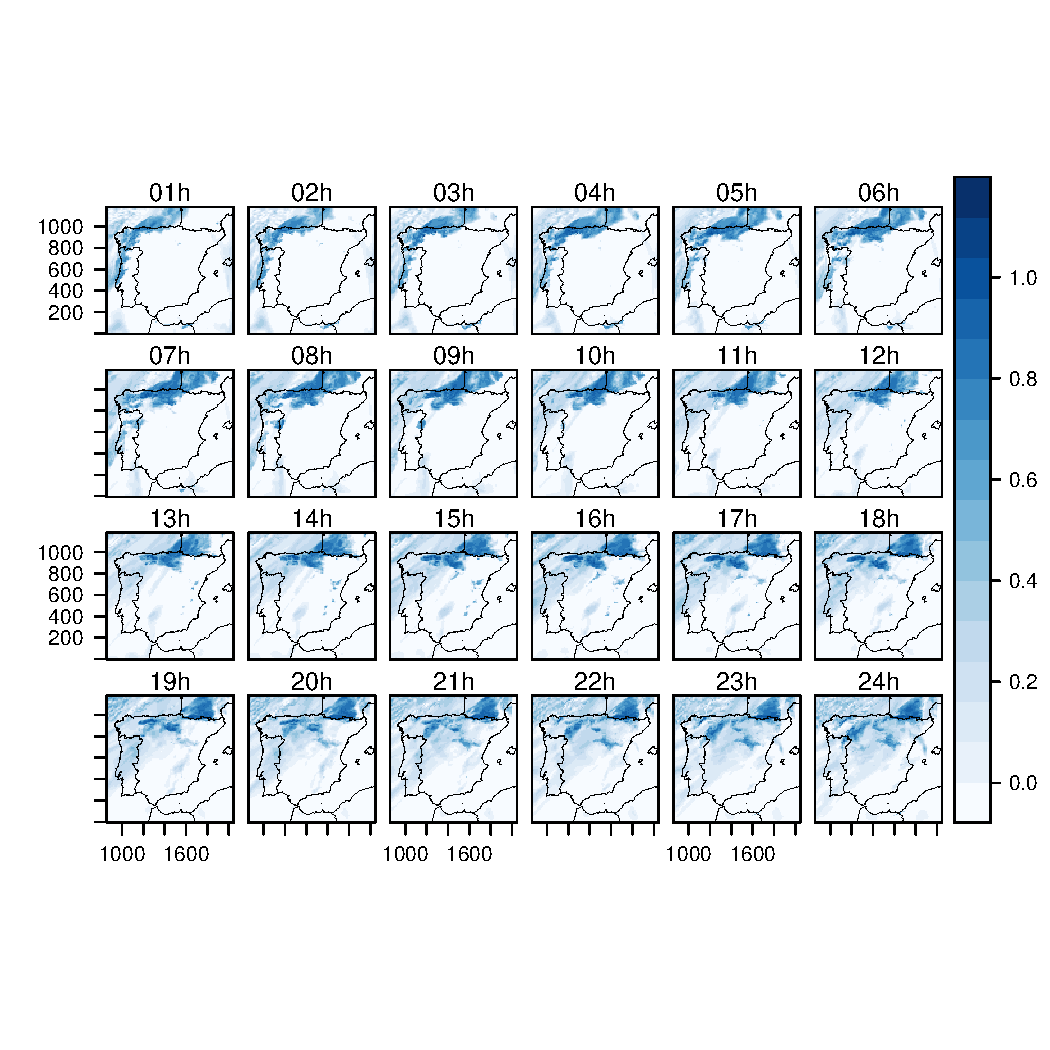
\includegraphics[width=.9\linewidth]{figs/cft.pdf}
\caption{\label{fig:cft}Forecast of hourly cloud cover at low and mid levels.}
\end{figure}

The movie and the static image are complementary tools and should be
used together. Watching the movie you will perceive the cloud transit
from Galicia to the Pyrenees gradually dissolving over the Cantabrian
region. On the other hand, with Figure \ref{fig:cft} you can locate the
position of a group of clouds in a certain hour and simultaneously
observe the relationship of that position with the evolution during
that period. With the movie you will concentrate your attention on the
movement. With small multiple pictures, your focus will be on
positions and relations. You should use both graphical tools to grasp
the entire 3D dataset.


\chapter{Spatiotemporal Point Observations}
\label{cha:pointsST}


\section{Introduction}
\label{sec-1}
Throughout this chapter we will revisit the data from the Integrated
Air Quality system of the Madrid City Council (section
\ref{sec:airQualityData}) to illustrate visualization methods
applicable for point space-time data. This dataset comprises the time
series of measurements acquired at each station of the network
during 2011. In the section \ref{sec:bubble} the data were converted
from spatiotemporal data to spatial data, where the time
information was suppressed to display only the yearly average
values. In this chapter we will work with the whole space-time dataset
using the tools provided by the \texttt{spacetime} package
\cite{Pebesma2012}.
\section{Data and Spatial Information}
\label{sec-2}

The starting point is to retrieve the data and combine it with the
spatial and temporal information. The data are contained in the
\texttt{airQuality} \texttt{data.frame}, and the locations are in \texttt{airStations}, a
\texttt{data.frame} that is converted to a \texttt{SpatialPointsDataFrame} object
with the \texttt{coordinates} method.

\index{Data!Air quality in Madrid}
\index{Packages!sp@\texttt{sp}}
\index{read.csv2@\texttt{read.csv2}}

\lstset{language=R,numbers=none}
\begin{lstlisting}
library(sp)

## Spatial location of stations
airStations <- read.csv2('data/airStations.csv')
## rownames are used as the ID of the Spatial object
rownames(airStations) <- substring(airStations$Codigo, 7)
coordinates(airStations) <- ~ long + lat
proj4string(airStations) <- CRS("+proj=longlat +ellps=WGS84")
## Measurements data
airQuality <- read.csv2('data/airQuality.csv')
## Only interested in NO2 
NO2 <- airQuality[airQuality$codParam==8, ]
\end{lstlisting}

Each row of this \texttt{data.frame} corresponds to a measurement at one
of the stations during a day of the year (long format, following
the schema proposed in \cite{Pebesma2012}).

The \texttt{spacetime} package defines several classes for spatiotemporal
data inheriting the classes defined by the \texttt{sp} and \texttt{xts} packages.
In particular, the \texttt{STFDF}, a class for spatiotemporal data with full
space-time grids with \texttt{n} spatial locations and \texttt{m} times, requires a
\texttt{data.frame} with \texttt{n·m} rows, (spatial index moving fastest).  Thus,
we need to transform this structure to build a multivariate time
series where each station is a different variable (space-wide under
the schema of \cite{Pebesma2012}). The procedure is

\begin{itemize}
\item Add a column with the \texttt{POSIXct} time index.
\item Reshape the \texttt{data.frame} from long to wide format with
  \texttt{reshape}.
\item Define a multivariate time series with \texttt{zoo} (Figure
  \ref{fig:NO2zoo}).
\item Coerce this time series to a vector with \texttt{n·m} rows.
\end{itemize}

\index{reshape@\texttt{reshape}}
\index{Packages!zoo@\texttt{zoo}}
\index{Packages!spacetime@\texttt{spacetime}}
\index{STFDF@\texttt{STFDF}}

\lstset{language=R,numbers=none}
\begin{lstlisting}
library(zoo)
library(spacetime)

NO2$time <- with(NO2, ISOdate(year, month, day))
NO2wide <- reshape(NO2[,c('codEst', 'dat', 'time')],
		   idvar='time', timevar='codEst',
		   direction='wide')
NO2zoo <- zoo(NO2wide[,-1], NO2wide$time)

dats <- data.frame(vals=as.vector(t(NO2zoo)))
NO2st <- STFDF(airStations, index(NO2zoo), dats)
\end{lstlisting}
\section{Graphics with \texttt{spacetime}}
\label{sec-3}
The \texttt{stplot} function of the \texttt{spacetime} package supplies the main
visualization methods for spatiotemporal data. When the mode \texttt{xy} is
chosen (default) it is mainly a wrapper around \texttt{spplot} and displays a
panel with the spatial data for each element of the time index (Figure
\ref{fig:NO2STxy}). The problem with this approach is that only a limited
number of panels can be correctly displayed on one page. In this
example, we print the first 12 days of the sequence.

\index{stplot@\texttt{stplot}}
\index{colorRampPalette@\texttt{colorRampPalette}}

\lstset{language=R,numbers=none}
\begin{lstlisting}
airPal <- colorRampPalette(c('springgreen1', 'sienna3', 'gray5'))(5)

stplot(NO2st[, 1:12], cuts=5, col.regions=airPal, edge.col='black')
\end{lstlisting}

\begin{figure}[htb]
\centering
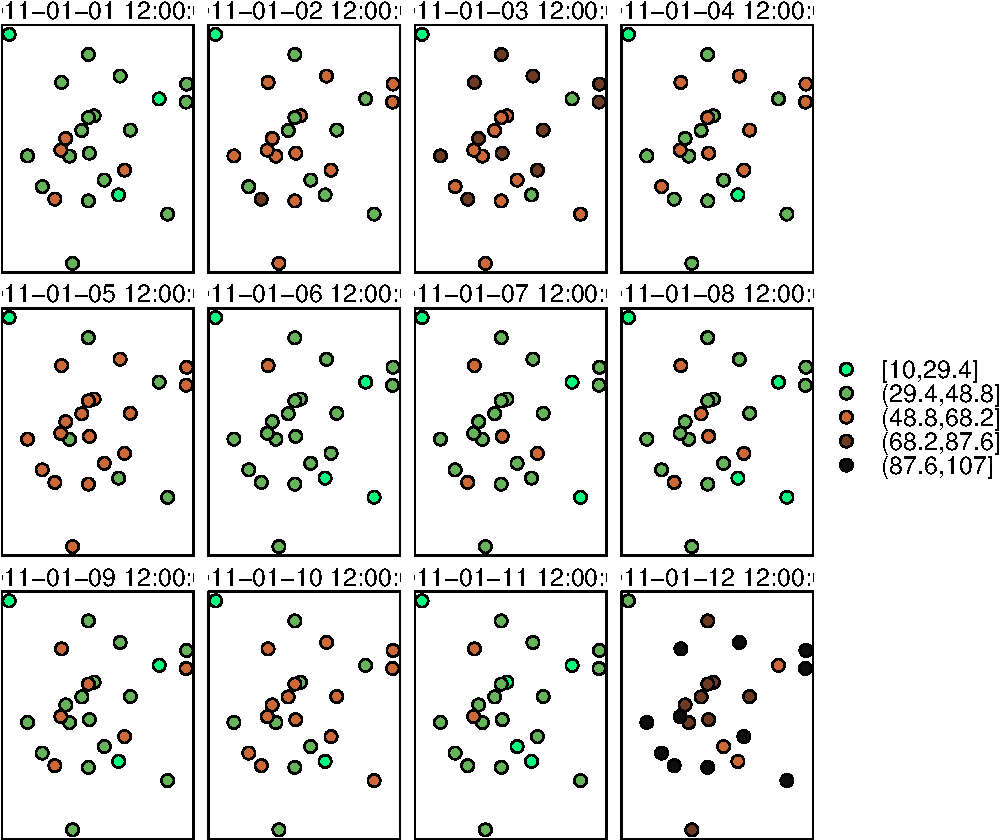
\includegraphics[width=.9\linewidth]{figs/NO2STxy.pdf}
\caption{\label{fig:NO2STxy}Scatterplots of the $NO_2$ values (2011) with a panel for each day of the time series. Each circle represents a different station.}
\end{figure}

With the mode \texttt{xt}, a space-time plot with space on the x-axis and
time on the y-axis is plotted (Figure \ref{fig:NO2hovmoller}).

\lstset{language=R,numbers=none}
\begin{lstlisting}
stplot(NO2st, mode='xt', col.regions=colorRampPalette(airPal)(15),
       scales=list(x=list(rot=45)), ylab='', xlab='')
\end{lstlisting}

\begin{figure}[htb]
\centering
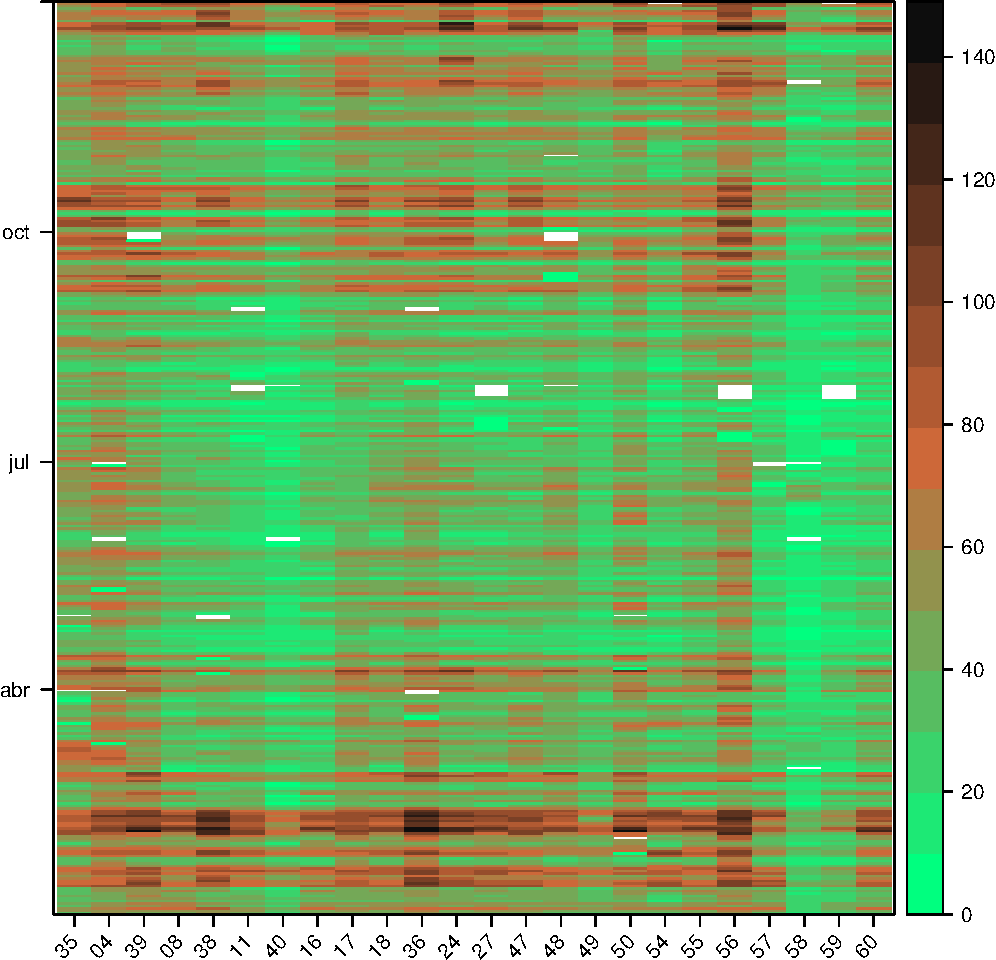
\includegraphics[width=.9\linewidth]{figs/NO2hovmoller.pdf}
\caption{\label{fig:NO2hovmoller}Space-time graphic of the NO\_2 time series. Each column represents a different station (denoted with the last two digits of the code).}
\end{figure}

Finally, with the mode \texttt{ts}, data are coerced to a multivariate time series
that is displayed in a single plot (Figure \ref{fig:NO2zoo}).

\lstset{language=R,numbers=none}
\begin{lstlisting}
stplot(NO2st, mode='ts', xlab='',
       lwd=0.1, col='black', alpha=0.6,
       auto.key=FALSE)
\end{lstlisting}

\begin{figure}[htb]
\centering
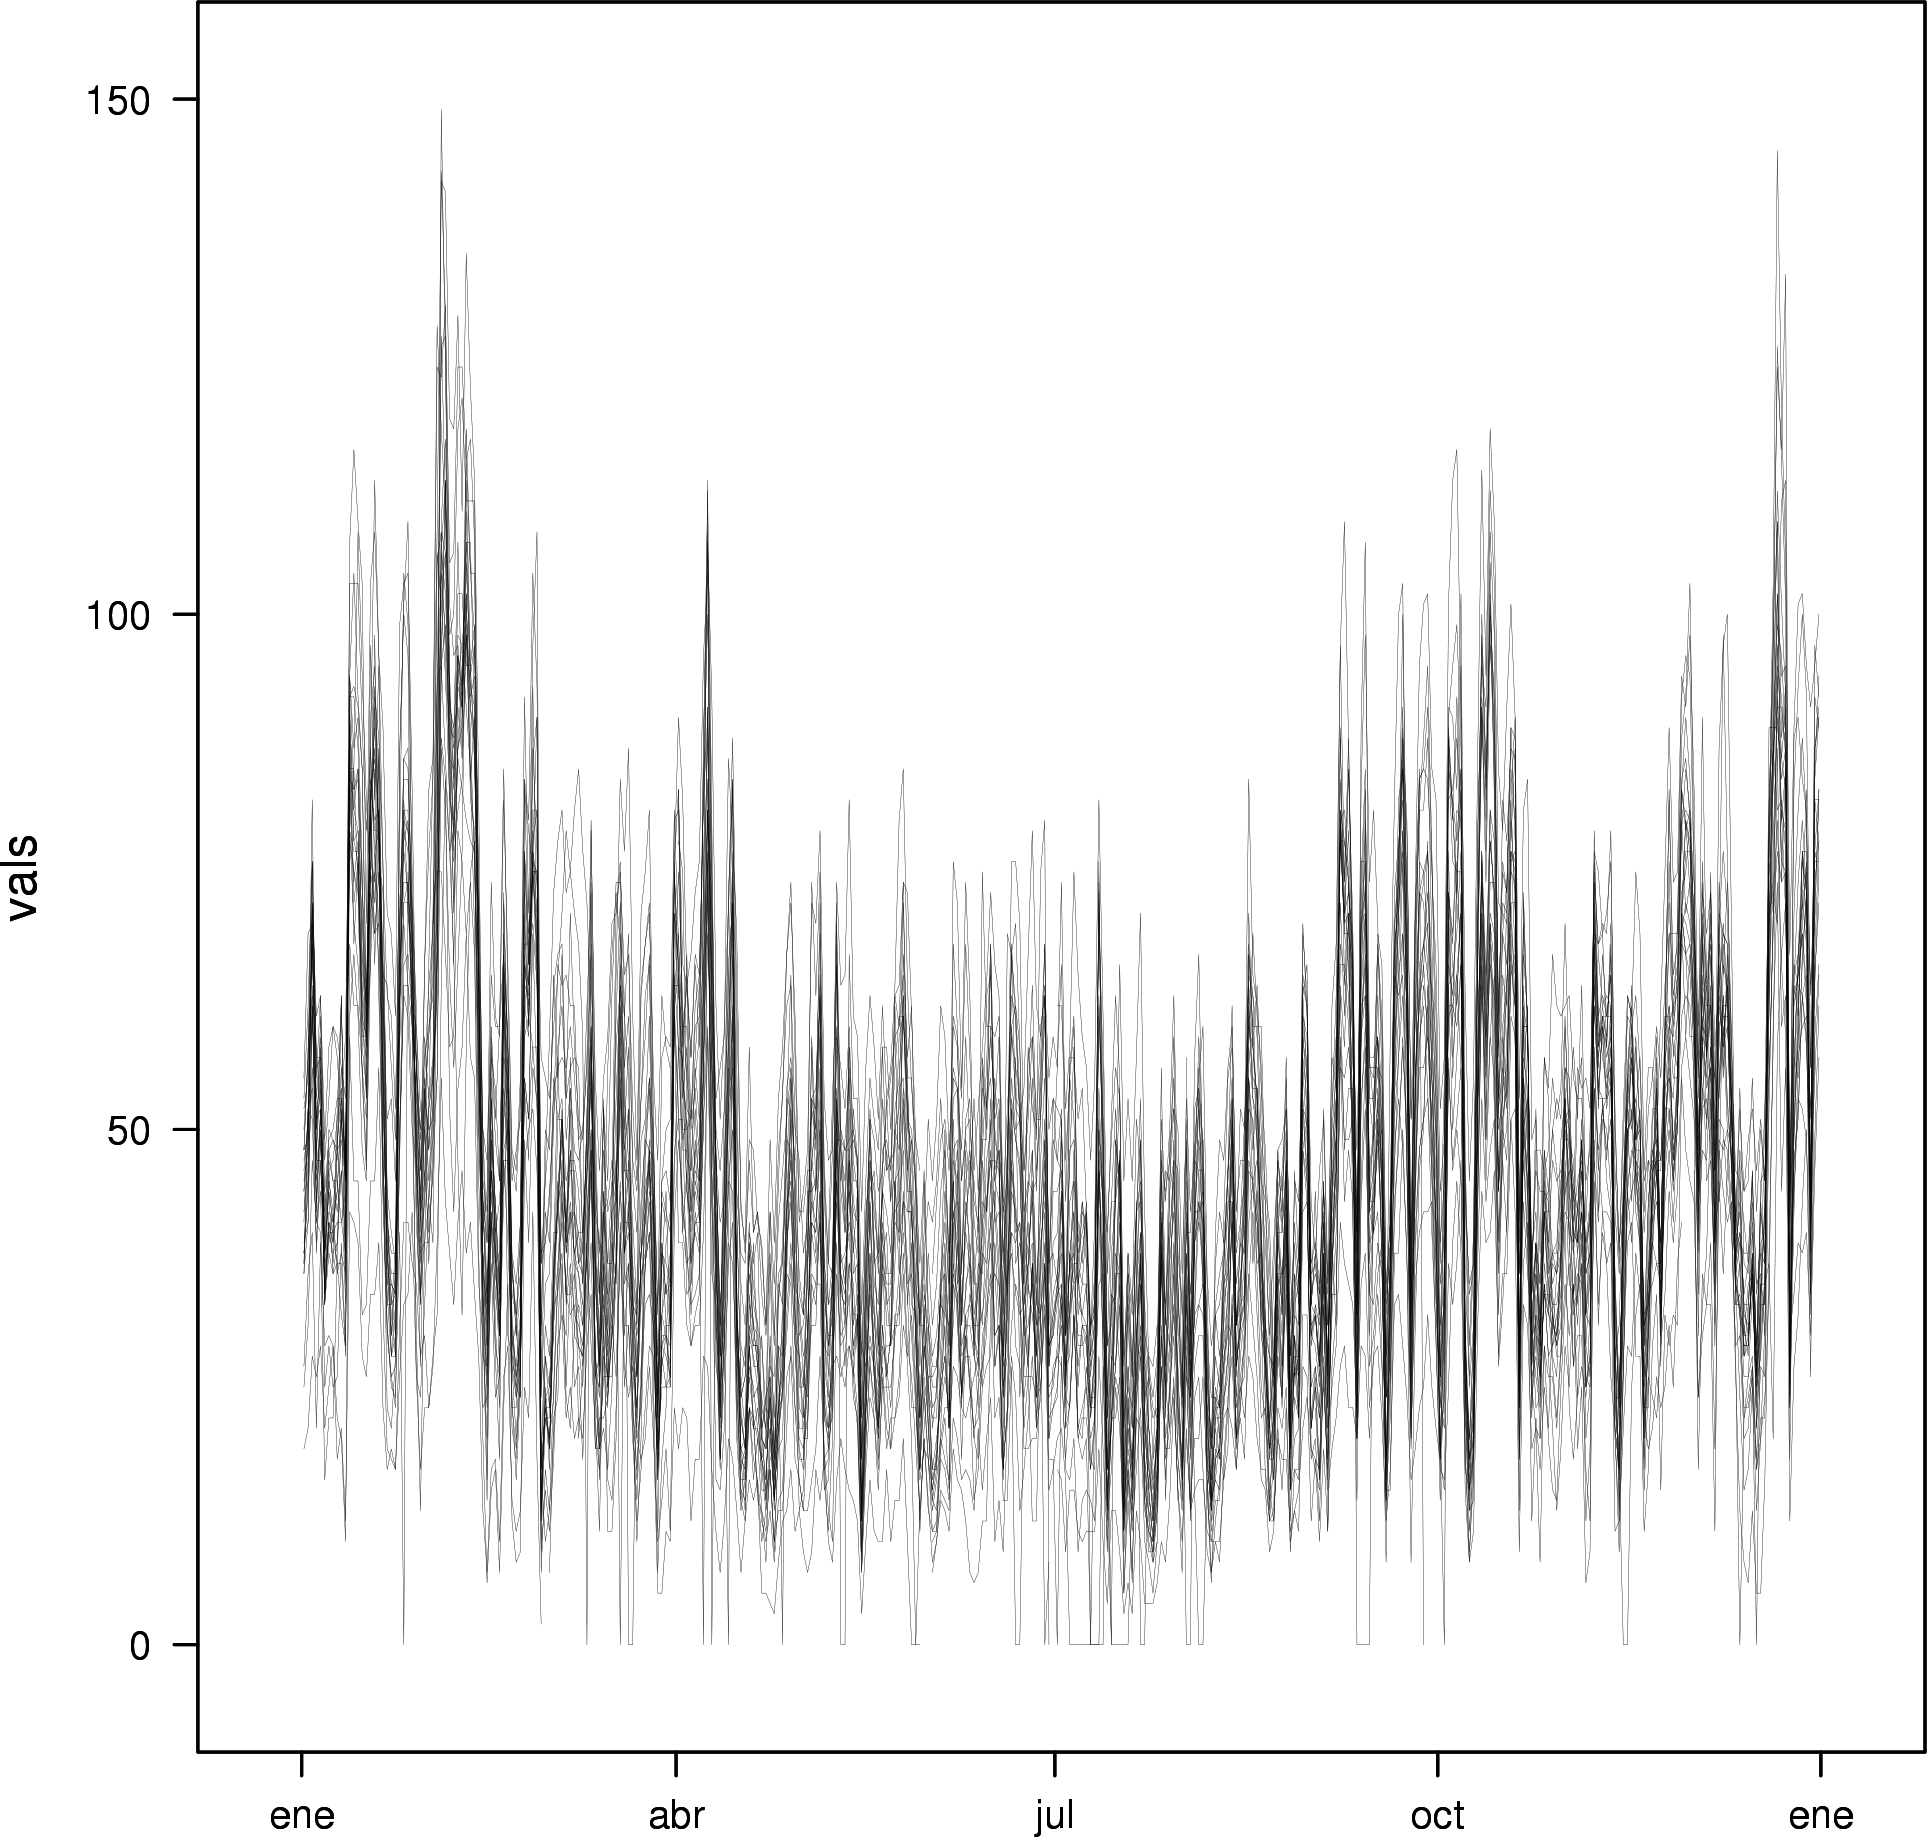
\includegraphics[width=.9\linewidth]{figs/NO2zoo.png}
\caption{\label{fig:NO2zoo}Time graph of the $NO_2$ time series (2011). Each line represents a different station.}
\end{figure}

These three graphics complement each other and together provide a more
complete view of the behavior of the data. For example in Figure
\ref{fig:NO2STxy}, we can find stations whose levels remain almost constant
throughout the 12-day period (namely, El Pardo-28079058\footnote{Use Figure \ref{fig:airMadrid} as reference of the
positions and codes of the stations.}, the
station at the top-left corner that is far from the city center),
while others fluctuate notably during this same period (for example,
Barajas-28079027 and Urb. Embajada-28079055, the two nearby stations
at the right). On the other hand, Figure \ref{fig:NO2hovmoller} loses the
spatial information but gives a more comprehensive view of the
evolution of the network. The station El Pardo-28079058 is
significantly below the rest of the stations during the whole year,
with the station Pza. Fdez Ladreda-28079056 being the opposite. In
between, the stations could be divided into two or three groups
according to their levels. Regardless, the group of stations reaches
maximum values during the first days of autumn and at the end of
winter. These maxima are clearly displayed in Figure \ref{fig:NO2zoo}.

\section{\floweroneleft Animation}
\label{sec-4}
Another approach for displaying this spatiotemporal data is using
animation. Once again, we will take advantage of the functionalities
of the \texttt{gridSVG} package.

\subsection{Initial Snapshot}
\label{sec-4-1}
The first step is to define the initial parameters of the animation:
starting values and duration.

\index{Packages!gridSVG@\texttt{gridSVG}}

\lstset{language=R,numbers=none}
\begin{lstlisting}
library(gridSVG)
## Initial parameters
start <- NO2st[,1]
## values will be encoded as size of circles,
## so we need to scale them
startVals <- start$vals/5000

nStations <- nrow(airStations)
days <- index(NO2zoo)
nDays <- length(days)
## Duration in seconds of the animation
duration <- nDays*.3
\end{lstlisting}

The first snapshot of the data is produced with \texttt{spplot}. We define an
auxiliary function, \texttt{panel.circlesplot}, to display the data encoding
values with circles of variable size and color.  This function
uses \texttt{grid.circle} from the \texttt{grid} package.  

The subsequent frames of the animation will modify the colors and
sizes of the circles according to the \texttt{NO2st} object.

\index{Packages!grid@\texttt{grid}}
\index{grid.circle@\texttt{grid.circle}}
\index{spplot@\texttt{spplot}}

\lstset{language=R,numbers=none}
\begin{lstlisting}
library(grid)

## Auxiliary panel function to display circles
panel.circlesplot <- function(x, y, cex, col='gray',
			      name='stationsCircles', ...){
grid.circle(x, y, r=cex,
	    gp=gpar(fill=col, alpha=0.5),
	    default.units='native', name=name)
}

pStart <- spplot(start, panel=panel.circlesplot,
		 cex=startVals,
		 scales=list(draw=TRUE), auto.key=FALSE)
pStart
\end{lstlisting}
\subsection{Intermediate States to Create the Animation}
\label{sec-4-2}
From this initial state, \texttt{grid.animate} creates a collection of
animated graphical objects with the intermediate states defined by
\texttt{animUnit} and \texttt{animValue}.  As previously stated, the $NO_2$ values
will be encoded with the radius of each circle, and the color of the
circles will distinguish between weekdays and weekend.  The use of
\texttt{rep=TRUE} ensures that the animation will be repeated indefinitely.

\index{animValue@\texttt{animValue}}
\index{animUnit@\texttt{animUnit}}
\index{grid.animate@\texttt{grid.animate}}

\lstset{language=R,numbers=none}
\begin{lstlisting}
## Color to distinguish between weekdays ('green')
## and weekend ('blue')
isWeekend <- function(x) {format(x, '%w') %in% c(0, 6)}
color <- ifelse(isWeekend(days), 'blue', 'green')
colorAnim <- animValue(rep(color, each=nStations),
		       id=rep(seq_len(nStations), nDays))

## Intermediate sizes of the circles
vals <- NO2st$vals/5000
vals[is.na(vals)] <- 0
radius <- animUnit(unit(vals, 'native'),
		       id=rep(seq_len(nStations), nDays))                     

## Animation of circles including sizes and colors
grid.animate('stationsCircles',
	     duration=duration,
	     r=radius,
	     fill=colorAnim,
	     rep=TRUE)
\end{lstlisting}
\subsection{Time Reference: Progress Bar}
\label{sec-4-3}
Information from an animation is better understood if a time
reference is included, for example with a progress bar.  The following
code builds a progress bar with ticks at the first day of each
month, and with color changing from gray (background) to blue as
the time advances.  On the other hand, it is convenient to provide
a method so the user can stop and restart the animation sequence
if desired.  This functionality is added with the definition of
two events, \texttt{onmouseover} and \texttt{onmouseout}, included with the
\texttt{grid.garnish} function.

\index{grid.rect@\texttt{grid.rect}}
\index{grid.text@\texttt{grid.text}}
\index{grid.animate@\texttt{grid.animate}}
\index{grid.segments@\texttt{grid.segments}}
\index{grid.garnish@\texttt{grid.garnish}}

\lstset{language=R,numbers=none}
\begin{lstlisting}
## Progress bar
prettyDays <- pretty(days, 12)
## Width of the progress bar
pbWidth <- .95
## Background
grid.rect(.5, 0.01, width=pbWidth, height=.01,
	  just=c('center', 'bottom'),
	  name='bgbar', gp=gpar(fill='gray'))

## Width of the progress bar for each day
dayWidth <- pbWidth/nDays
ticks <- c(0, cumsum(as.numeric(diff(prettyDays)))*dayWidth) + .025
grid.segments(ticks, .01, ticks, .02)
grid.text(format(prettyDays, '%d-%b'),
		 ticks, .03, gp=gpar(cex=.5))
## Initial display of the progress bar
grid.rect(.025, .01, width=0,
	  height=.01, just=c('left', 'bottom'),
	  name='pbar', gp=gpar(fill='blue', alpha='.3'))
## ...and its animation
grid.animate('pbar', duration=duration,
	     width=seq(0, pbWidth, length=duration),
	     rep=TRUE)
## Pause animations when mouse is over the progress bar
grid.garnish('bgbar',
	     onmouseover='document.rootElement.pauseAnimations()',
	     onmouseout='document.rootElement.unpauseAnimations()')
\end{lstlisting}

The SVG file is finally produced with \texttt{gridToSVG} (Figure \ref{fig:NO2pb})

\index{grid.export@\texttt{grid.export}}  

\lstset{language=R,numbers=none}
\begin{lstlisting}
grid.export('figs/NO2pb.svg')
\end{lstlisting}

\begin{figure}
  \centering
  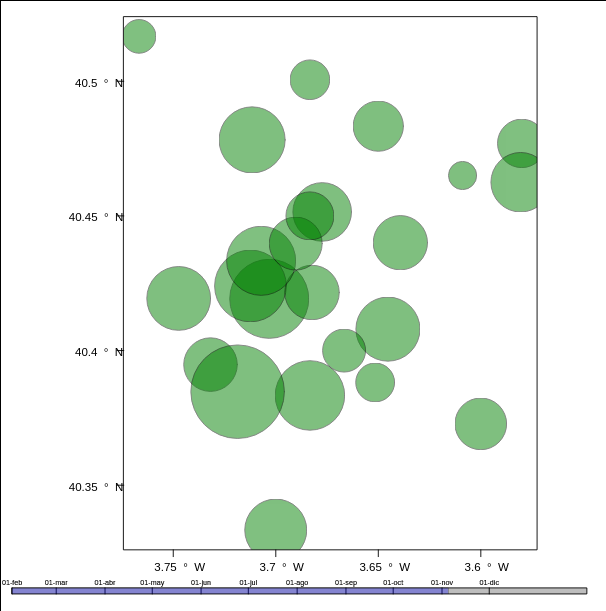
\includegraphics[width=\textwidth]{figs/NO2pb.png}
  \caption{Animated circles of the $NO_2$ space-time data with a progress bar.}
  \label{fig:NO2pb}
\end{figure}
\subsection{Time Reference: A Time Series Plot}
\label{sec-4-4}
A different and more informative solution is to add a time series
plot instead of a progress bar.  This time series plot displays
the average value of the set of stations, with a point and a
vertical line to highlight the time position as the animation
advances (Figure \ref{fig:vLine}).
\lstset{language=R,numbers=none}
\begin{lstlisting}
## Time series with average value of the set of stations
NO2mean <- zoo(rowMeans(NO2zoo, na.rm=TRUE), index(NO2zoo))
## Time series plot with position highlighted
pTimeSeries <- xyplot(NO2mean, xlab='', identifier='timePlot') +
    layer({
	grid.points(0, .5, size=unit(.5, 'char'),
		    default.units='npc',
		    gp=gpar(fill='gray'),
		    name='locator')
	grid.segments(0, 0, 0, 1, name='vLine')
    })

print(pStart, position=c(0, .2, 1, 1), more=TRUE)
print(pTimeSeries, position=c(.1, 0, .9, .25))
\end{lstlisting}


Once again, \texttt{grid.animate} creates a sequence of intermediate states
for each object of the graphical scenes: The signaling point and
vertical line follow the time evolution, while the sizes and colors of
each station circle change as in the previous approach.  Moreover, the
\texttt{onmouseover} and \texttt{onmouseout} events are defined with \texttt{grid.garnish}
so the user can pause and restart the animation by hovering the mouse
over the time series plot.
\lstset{language=R,numbers=none}
\begin{lstlisting}
grid.animate('locator',
	     x=unit(as.numeric(index(NO2zoo)), 'native'),
	     y=unit(as.numeric(NO2mean), 'native'),
	     duration=duration, rep=TRUE)

xLine <- unit(index(NO2zoo), 'native')

grid.animate('vLine',
	     x0=xLine, x1=xLine,
	     duration=duration, rep=TRUE)

grid.animate('stationsCircles',
	     duration=duration,
	     r=radius,
	     fill=colorAnim,
	     rep=TRUE)

## Pause animations when mouse is over the time series plot
grid.garnish('timePlot', grep=TRUE,
	     onmouseover='document.rootElement.pauseAnimations()',
	     onmouseout='document.rootElement.unpauseAnimations()')

grid.export('figs/vLine.svg')
\end{lstlisting}


\begin{figure}
  \centering
  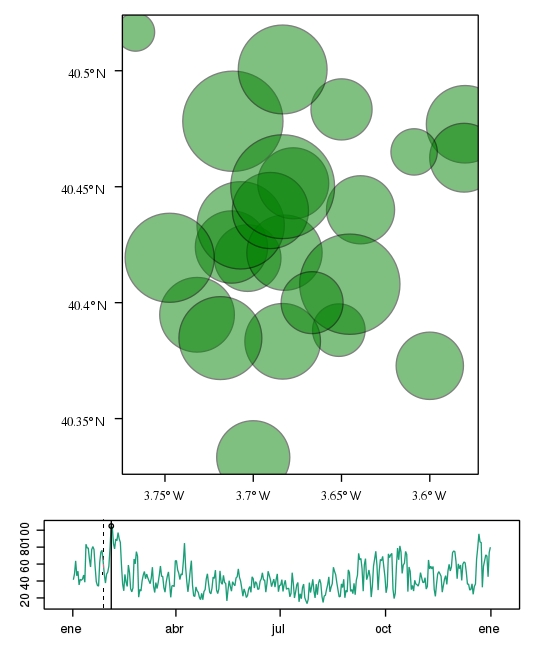
\includegraphics[width=\textwidth]{figs/vLine.png}
  \caption{Animated circles of the $NO_2$ space-time data with a a time series as reference.}
  \label{fig:vLine}
\end{figure}



%%% Local Variables:
%%% TeX-master: "../main.tex"
%%% End: